\documentclass[12pt, letterpaper]{article}
\usepackage[utf8]{inputenc}
\usepackage{graphicx}
\usepackage{amsmath}

\title{Creating a Test Statistic to Find if the Number of Misses in a Song from Guitar Hero is Random}
\author{Shannon Coyle, Samantha Colucci, and Brianna Cirillo}
\date{December 2020}

\begin{document}
\maketitle

\section{INTRODUCTION}
The game, Guitar Hero, collects information regarding the number of “hits” recorded by the player.  This poses the question about the randomness of the misses in a song and if they are correlated to the difficulty of the part of the song.

The study investigates the randomness of different songs using varying methods.  These methods looked at the number of miss streaks over the total number of misses, distances between each miss, and using the runs test.  The resampling of the data sets was performed through parametric bootstrapping, permutation tests, and regular bootstrapping. Using resampling and our methods together allowed us to assess the randomness of a given song based on the results. 

This report explains the methodology used in order to test the randomness of a song. The methods and resampling used throughout the project gave results for the empirical type 1 error and the power of the test. These methods were applied to different songs, therefore, returning different results. This report will also look at the limitations and future ideas for the project, and how some of our methods worked well while others did not.

\section{METHODOLOGY}
\subsection{Method 1}
The first method looks at the proportion of the number of miss streaks over the number of total misses.  A streak was definied as one or more misses in a row since it was easier with the code and some samples did not have that many streaks to look at.  From this method, we discovered that the proportion does not tell us anything about the location of the misses.  This proved to be difficult to determine randomness of misses without knowing the exact location of them.  

\subsection{Method 2}
The second method calculates the distances between misses in a song.  The idea behind this method was that if we can see where the misses are occurring, we can see if they are random.  We can seeing where the distances are occuring randomly and conclude that the misses must also be occurring randomly. 

There was an attempt to use a median distance as a basis rather than the mean because the distances were varied, so the average would not tell us that much.  This led to a problem because a lot of the songs had long miss streaks, which lead to a distance of 0, so the median would also become zero.  With this small issue, it led to the idea of use the runs test on this method and, therefore, the distances.  

\subsection{Runs Test}
Knowing that the runs test is a preconceived test for randomness, the idea behind using this was to use it on the distances of misses within a song, rather than just using it on the song. As mentioned previously if a conclusion can be reached that the distances are random, this would imply randomness of the misses in the song. 

A run is defined as a series of increasing or decreasing values, while the number of values in each series is the length of each run. The number of runs in a data set, denoted R, is crucial because this is the number that is used to derive the test statistic. The other values involved in deriving the test statistics is the expected number of runs, denoted $\overline{R}$, the median value of the data sample, the standard deviation of the number of runs, and the number of values below and above the median. 

Once the test statistic is derived, the runs test comes to a conclusion about whether or not to reject the null hypothesis. Here, the test defines: 


The runs test program used was found from the snpar package in RStudio. A p-value, the number of runs and an alternative hypothesis of nonrandomness is produced once the test is run. This package was specifically chosen because was created to be used on discrete data, rather than continuous. When using this method, each song was resampled and a distance vector for each sample was computed. The runs test was then used on the distances to determine if the null hypothesis of randomness should be rejected or not. 

\subsection{Resampling Methods}
\subsubsection{Parametric Bootstrap}
The Parametric Bootstrap was used to generate a bootstrap using a parameterized distribution.  It takes in a specified number of resamples then performs a Bernoulli distribution in order to resample the data.  The Bernoulli distribution looks at the sample size then the event probability, which was set to 50\% since the data is composed of 0's and 1's.  This goes through and resamples the data as either a 0 or a 1 for the specified number of resamples that was initialized.   

\subsubsection{Permutation Resampling}
The permutation resampling method is a type of randomization that was developed for data that does not conform to the assumptions needed to perform the statistical method desired. There are multiple advantages to using this type of resampling. In order to implement this, one does not need to know the distribution of the data and it can also be used on small sample sizes. A major disadvantage to using this method is the amount of computer power it takes, since as the sample size begins to increase, the number of permutations computed during the resampling increases rapidly. For this reason, when the permutation resampling is used throughout Methods 1, 2 and the Runs test, the amount of samples produced by this resampling is smaller than that produced by the other resampling techniques.

The main element of this resampling method, that differentiates it from most other methods, is that it resamples *without* replacement. Essentially, it redistributes the original elements of the data in a different order. Though this sampling can be beneficial to use here since the distribution of our data is unknown, it also presents issues when checking for randomness. For example, if there is a detectable pattern in a specific song or sample, the permutation resampling may cause the presence of that pattern to disappear, due to the way the resampling is done. When this became an issue during the research, a different approach was taken to ensure that if the songs being analyzed do have a pattern, that pattern is not lost. This is discussed more in the Power of the Test section. 

\subsubsection{Regular Bootstrap}


\section{EMPIRICAL TYPE 1 ERROR AND POWER SIMULATIONS}
To look into the empirical type 1 error rates, random songs were created. In order to create the songs,a sample of 50 observations were taken from a binomial distribution with a probability of 0.5. The songs were reampled using each of the aforementioned methods. The distances of misses in the reampled sample, were then calculated. The runs test was then performed on these distances for each alpha from 0.001 to 0.1 that were incremented at 0.005. This therefore returned the average of the p-values that were less that 0.05 for each theoretical alpha. 

For the final power simulations, different scenarios were used in order to create a song that is not random. This means that the songs created should make the null hypothesis false. Doing this will show how well the metrics identify nonrandomness.The scenarios using positive pairwise correlation generated two songs, one with 200 notes and one with 600 notes. The probability model used was that the probability of missing a note was 0.2 and the correlation between any two consecutive notes was 0.3.The scenarios using blocks with different difficulties also created two songs, one with 200 notes and one with 600 notes. For each song created using this scenario, there were easy, medium, hard, and very hard sections. The probability of missing a note in an easy section is 0.01, in a medium section is 0.05, in a hard section 0.25, and in a very hard section is 0.5. The scenarios using the autoregressive model of order 1 generated six songs, three with 200 notes and three with 600 notes. The probability model used for the first type is the probability of missing a note is 0.1 and the correlation between any two notes is $0.5^{\mid i-j \mid}$. For the probability model for the second type, the proability of missing a note stayed 0.1, but the correlation between any two notes is $0.3^{\mid i-j \mid}$. For the third type, the probability of missing a note is 0.2 and the correlation between any two notes is $0.5^{\mid i-j \mid}$.

\subsection{Parametric Bootstrap}
When resampling with a parametric bootstrap, multiple simulations were run with a varying number of observations - it was usually 50 or 100 observations.  

\subsubsection{Empirical Type 1 Error} 
To calculate the empirical type 1 error rate, the parametric bootstrap worked better with 50 observations as opposed to 100 observations.  There were also two random songs made to see how the error rate varies between songs.  These random songs were generated through code in which they were both 50 notes long and had a 50\% chance of being a 0 or a 1.  Alpha was increased by 0.01, but error rates between 0.005 and 0.001 ended up being 0.00. 

\begin{tabular}{|c|c|c|}
\hline
\textbf{Alpha} & \textbf{Empirical - Random Song 1} & \textbf{Empirical - Random Song 2} \\
\hline
$\alpha = 0.001$ & 0.00 & 0.00\\
$\alpha = 0.005$ &  0.01 & 0.00\\
$\alpha = 0.006$ &  0.01 & 0.02\\
$\alpha = 0.007$ & 0.01 & 0.02\\
$\alpha = 0.008$ & 0.01 & 0.04\\
$\alpha = 0.009$ & 0.01 & 0.04\\
$\alpha = 0.01$ & 0.01 & 0.04\\
$\alpha = 0.02$ & 0.01 & 0.04\\
$\alpha = 0.03$ & 0.01 & 0.06\\
$\alpha = 0.04$ & 0.01 & 0.06\\
$\alpha = 0.05$ &  0.03 & 0.07\\
$\alpha = 0.06$ &  0.06 & 0.08\\
$\alpha = 0.07$ &  0.08 & 0.09\\
$\alpha = 0.08$ &  0.08 & 0.13\\
$\alpha = 0.09$ & 0.08 & 0.13\\
$\alpha = 0.1$ & 0.08 & 0.14\\
\hline
\end{tabular} \\

The table above shows the difference between the two random songs and how the second random song displayed more of a variation of error values.  The second random song showed to have more of a curve and varying error rates, whereas, the first random song had multiple occurrences of the same p-value for different alphas. 

\begin{figure}[!hb]
\centering
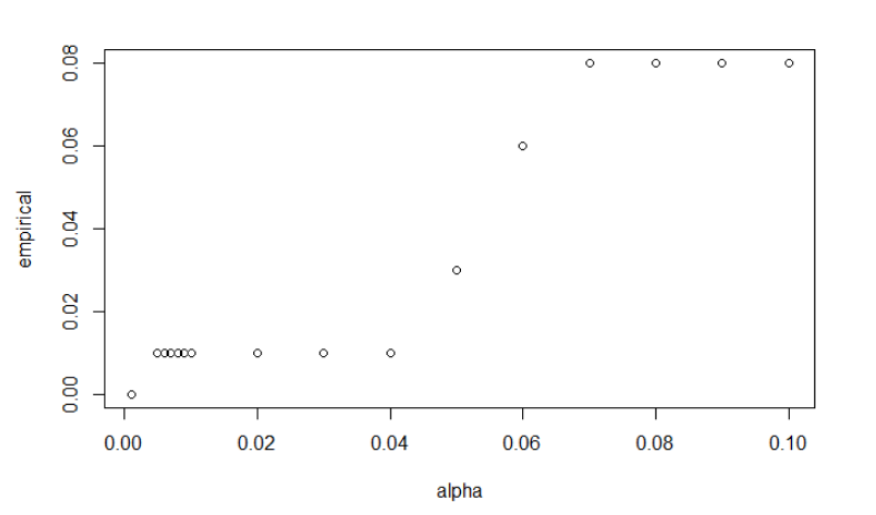
\includegraphics[width=10cm]{Type1_Song1.png}
\caption{Graph of Type 1 error rates for Random Song 1 with 50 observations}
\label{fig: Type 1 Error, Song 1, n=50}
\end{figure}

\begin{figure}[!hb]
\centering
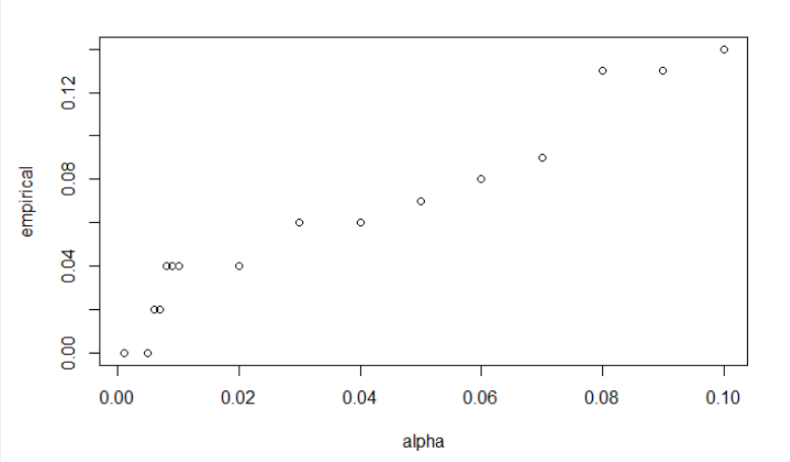
\includegraphics[width=10cm]{Type1_Song2.png}
\caption{Graph of Type 1 error rates for Random Song 2 with 50 observations}
\label{fig: Type 1 Error, Song 2, n=50}
\end{figure}


\subsubsection{Final Power Simulations}
When using the Parametric Bootstrap to return a power, they were generally very low p-values or 0.  The power was always equal to 0 when alpha was set to 0.001 and many of the scenarios gave 0 for every value of alpha.  There were three scenarios that gave actual values which were the both blocks methods and the autoregressive model of order 1 that had 200 notes per song, a probability of missing a note as p=0.1, and $\rho = 0.3$. \\

\begin{tabular}{|c|c|c|c|c|c|}
\hline
\textbf{Type 1 Error Rate Scenario} & $\alpha = 0.001$ &  $\alpha = 0.005$ &  $\alpha = 0.01$ &  $\alpha = 0.05$ &  $\alpha = 0.10$ \\
\hline
Neg. Pair Correlation, n = 200 & 0.00 & 0.00 & 0.00 & 0.00 & 0.00 \\
\hline
Neg. Pair Correlation, n = 600 & 0.00 & 0.00 & 0.00 & 0.00 & 0.00 \\
\hline
Blocks, n = 200 & 0.00 & 0.03 & 0.03 & 0.11 & 0.30 \\
\hline
Blocks, n = 600 & 0.00 & 0.00 & 0.01 & 0.02 & 0.08 \\
\hline
AR(1), p=0.1, $\rho = 0.5$, n = 200 & 0.00 & 0.00 & 0.00 & 0.00 & 0.00 \\
\hline
AR(1), p=0.1, $\rho = 0.5$, n = 600 & 0.00 & 0.00 & 0.00 & 0.00 & 0.00 \\
\hline
AR(1), p=0.1, $\rho = 0.3$, n = 200 & 0.00 & 0.00 & 0.00 & 0.01 & 0.01 \\
\hline
AR(1), p=0.1, $\rho = 0.3$, n = 600 & 0.00 & 0.00 & 0.00 & 0.00 & 0.00 \\
\hline
AR(1), p=0.2, $\rho = 0.5$, n = 200 & 0.00 & 0.00 & 0.00 & 0.00 & 0.00 \\
\hline
AR(1), p=0.2, $\rho = 0.5$, n = 600 & 0.00 & 0.00 & 0.00 & 0.00 & 0.00 \\
\hline
\end{tabular} \\

From the table, it is evident that most of the values obtained are 0 with exceptions for three of the scenarios.  Aside from the table, the graphs also show the large number of occurrences of 0 as a power.

\begin{figure}[!hb]
\centering
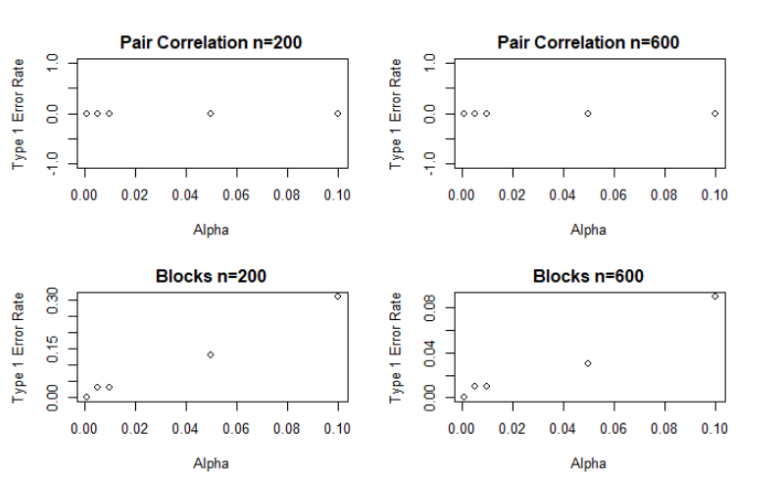
\includegraphics[width=10cm]{PowerGraphs1.png}
\caption{Graph of first four scenarios to calculate the power of a test}
\label{fig: Power Graphs 1}
\end{figure}

\begin{figure}[!hb]
\centering
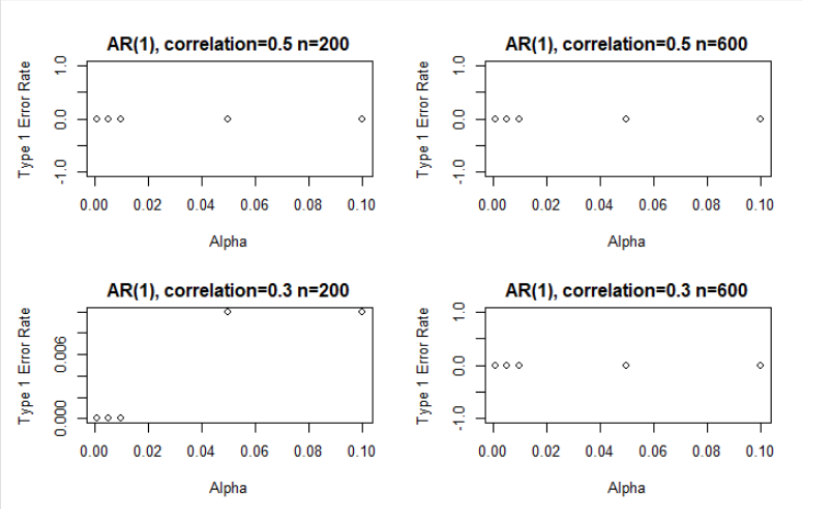
\includegraphics[width=10cm]{PowerGraphs2.png}
\caption{Graph of last four scenarios to calculate the power of a test}
\label{fig: Power Graphs 2}
\end{figure}


\subsection{Permutation Test}
\subsection{Non-Parametric Bootstrap}
\subsubsection{Empirical Type 1 Error} 
By taking 50 samples from the binomial distribution, the resulting random song was:
\begin{gather*}
  0 1 0 0 0 1 0 0 1 1 0 1 0 1 1 1 1 1 1 1 0 
  1 0 0 1 1 0 0 1 0 0 1 0 0 0 1 0 1 0 1 0 0
  0 1 0 1 1 1 1 0
\end{gather*} 
To resample the data, the nonparametric bootstrap was used and the song was resampled 100 times. The runs test was then performed on the distances of misses in the bootstrapped sample. This returned the average of the p-values that were less that 0.05 for each theoretical alpha, whis can be seen in the table below.
\begin{table}[t]
\begin{center}
\begin{tabular}{|c|c|}
\textbf{Type 1 Error} & \textbf{Random Song 1}\\
$\alpha = 0.001$ & 0.00\\
$\alpha = 0.005$ &  0.00\\
$\alpha = 0.006$ &  0.00\\
$\alpha = 0.007$ & 0.00\\
$\alpha = 0.008$ & 0.02\\
$\alpha = 0.009$ & 0.02\\
$\alpha = 0.01$ & 0.02\\
$\alpha = 0.02$ & 0.03\\
$\alpha = 0.03$ & 0.03\\
$\alpha = 0.04$ & 0.05\\
$\alpha = 0.05$ &  0.05\\
$\alpha = 0.06$ &  0.05\\
$\alpha = 0.07$ &  0.05\\
$\alpha = 0.08$ &  0.06\\
$\alpha = 0.09$ & 0.07\\
$\alpha = 0.1$ & 0.08 \\ 
\end{tabular}
\end{center}
\caption{A function was created to loop through p-values from 0.001 to 0.1 that incremented by 0.005, in order to  generate the Type 1 Error Rates. The table above shows the rates obtained with their respective alpha.}

\label{fig: Type 1 Error Rates for Nonparametric Bootstrap}
\end{table}

The empirical alpha seems to very roughly, match the theoretical alphas. Although, the empirical alphas were not increasing consistently. They would get stuck at certain alphas such as 0.02 and 0.05. Therefore, the theoretical alphas are increasing at a faster rate than the empirical alphas are.

\subsubsection{Final Power Simulations}
For the final power simulations, 
\begin{table}[t]
\begin{center}
\begin{tabular}{|c|c|c|c|c|c|}
\hline
\textbf{Type 1 Error Rate Scenario} & $\alpha = 0.001$ &  $\alpha = 0.005$ &  $\alpha = 0.01$ &  $\alpha = 0.05$ &  $\alpha = 0.10$ \\
\hline
Neg. Pair Correlation, n = 200 & 0.00 & 0.00 & 0.00 & 0.00 & 0.00 \\
\hline
Neg. Pair Correlation, n = 600 & 0.00 & 0.00 & 0.00 & 0.00 & 0.00 \\
\hline
Blocks, n = 200 & 0.00 & 0.04 & 0.04 & 0.04 & 0.04 \\
\hline
Blocks, n = 600 & 0.00 & 0.01 & 0.01 & 0.01 & 0.01 \\
\hline
AR(1), p=0.1, $\rho = 0.5$, n = 200 & 0.00 & 0.00 & 0.00 & 0.00 & 0.00 \\
\hline
AR(1), p=0.1, $\rho = 0.5$, n = 600 & 0.00 & 0.00 & 0.00 & 0.00 & 0.00 \\
\hline
AR(1), p=0.1, $\rho = 0.3$, n = 200 & 0.00 & 0.00 & 0.00 & 0.01 & 0.01 \\
\hline
AR(1), p=0.1, $\rho = 0.3$, n = 600 & 0.00 & 0.00 & 0.00 & 0.00 & 0.00 \\
\hline
AR(1), p=0.2, $\rho = 0.5$, n = 200 & 0.00 & 0.00 & 0.00 & 0.00 & 0.00 \\
\hline
AR(1), p=0.2, $\rho = 0.5$, n = 600 & 0.00 & 0.01 & 0.01 & 0.01 & 0.01 \\
\hline
\end{tabular}
\end{center}
\caption{The table shows the power at each theoretical alpha for each of the scenarios above.}
\label{fig: Power Simulations using Nonparametric Bootstrap}
\end{table}



\section{APPLICATION}
To obtain a p-value for each song, 100 bootstraps were performed to change the 0's and 1's to different orders and sequences.  Previously, 1000 bootstraps were being done, but it was taking a significant amount of time to return a p-value.  The null hypothesis being followed is that the songs are random and the alternative hypothesis is that the songs are not random. 

\subsection{Song 1: "Judith"}
\subsubsection{Parametric Bootstrap}
\begin{tabular}{|c|c|c|}
\hline
\textbf{Method Type} & P-Value \\
\hline
Method 1 & 0 \\
\hline
Runs Test & 0.512 \\ 
\hline
\end{tabular} \\
The p-value of the Method 1 test tells us to reject the null hypothesis while the Run tests p-value tells us to fail to reject the null hypothesis.

\subsubsection{Permutation Tests}

\subsubsection{Non-Parametric Bootstrap}
\begin{tabular}{|c|c|c|}
\hline
\textbf{Method Type} & P-Value \\
\hline
Method 1 & 0 \\
\hline
Runs Test & 0.998 \\ 
\hline
\end{tabular}

\subsection{Song 2: "Hurts"}
\subsubsection{Parametric Bootstrap}
\begin{tabular}{|c|c|c|}
\hline
\textbf{Method Type} & P-Value \\
\hline
Method 1 & 0  \\
\hline
Runs Test & 0.512 \\ 
\hline
\end{tabular} \\
The p-value of the Method 1 test tells us to reject the null hypothesis while the Run tests p-value tells us to fail to reject the null hypothesis.

\subsubsection{Nonparametric Bootstrap}
\begin{tabular}{|c|c|c|}
\hline
\textbf{Method Type} & P-Value \\
\hline
Method 1 & 0.186  \\
\hline
Runs Test & 0.459 \\ 
\hline
\end{tabular}

\subsection{Song 3: "American Girl"}
\subsubsection{Parametric Bootstrap}
\begin{tabular}{|c|c|}
\hline
\textbf{Method Type} & P-Value \\
\hline
Method 1 & 0.16 \\
\hline
Runs Test & 0.211 \\ 
\hline 
\end{tabular} \\
The p-value of the Method 1 test tells us to fail to reject the null hypothesis and the Run tests p-value tells us to fail to reject the null hypothesis as well.

\subsubsection{Nonparametric Bootstrap}
\begin{tabular}{|c|c|c|}
\hline
\textbf{Method Type} & P-Value \\
\hline
Method 1 & 0  \\
\hline
Runs Test & 0.841 \\ 
\hline
\end{tabular}

\subsection{Song 4: "Funky"}
\subsubsection{Parametric Bootstrap}
\begin{tabular}{|c|c|c|}
\hline
\textbf{Method Type} & P-Value \\
\hline
Method 1 & 0 \\
\hline
Runs Test & 0.08  \\ 
\hline
\end{tabular} \\
The p-value of the Method 1 test tells us to reject the null hypothesis while the Run tests p-value tells us to fail to reject the null hypothesis.

\subsubsection{Nonparametric Bootstrap}
\begin{tabular}{|c|c|c|}
\hline
\textbf{Method Type} & P-Value \\
\hline
Method 1 & 0  \\
\hline
Runs Test & 0.656 \\ 
\hline
\end{tabular}

\subsection{Song 5: "Ring of Fire"}
\subsubsection{Parametric Bootstrap}
\begin{tabular}{|c|c|c|}
\hline
\textbf{Method Type} & P-Value  \\
\hline
Method 1 & 2.204 $[e^{-16}]$ \\
\hline
Runs Test & 0.44 \\ 
\hline
\end{tabular} \\
The p-value of the Method 1 test tells us to reject the null hypothesis while the Run tests p-value tells us to fail to reject the null hypothesis.

\subsubsection{Nonparametric Bootstrap}
\begin{tabular}{|c|c|c|}
\hline
\textbf{Method Type} & P-Value \\
\hline
Method 1 & 0  \\
\hline
Runs Test & 0.317 \\ 
\hline
\end{tabular}

\subsection{Song 6: "Watchtower"}
\subsubsection{Parametric Bootstrap}
\begin{tabular}{|c|c|c|}
\hline
\textbf{Method Type} & P-Value  \\
\hline
Method 1 & 2.204 $[e^{-16}]$ \\
\hline
Runs Test & 0.66 \\ 
\hline
\end{tabular} \\
The p-value of the Method 1 test tells us to reject the null hypothesis while the Run tests p-value tells us to fail to reject the null hypothesis.

\subsubsection{Nonparametric Bootstrap}
\begin{tabular}{|c|c|c|}
\hline
\textbf{Method Type} & P-Value \\
\hline
Method 1 & 0  \\
\hline
Runs Test & 0.727 \\ 
\hline
\end{tabular}

\subsection{Song 7: "Wolf"}
\subsubsection{Parametric Bootstrap}
\begin{tabular}{|c|c|c|}
\hline
\textbf{Method Type} & P-Value  \\
\hline
Method 1 & 2.204 $[e^{-16}]$ \\
\hline
Runs Test & 0.58 \\ 
\hline
\end{tabular} \\
The Method 1 test says to reject the null hypothesis of randomness and the Runs test says to fail to reject the null hypothesis.

\subsubsection{Nonparametric Bootstrap}
\begin{tabular}{|c|c|c|}
\hline
\textbf{Method Type} & P-Value \\
\hline
Method 1 & 0.02  \\
\hline
Runs Test & 0.727 \\ 
\hline
\end{tabular}


\section{DISCUSSION/LIMITATIONS/IDEAS FOR FURTHER RESEARCH}

\section{APPENDIX}

\begin{figure}[!hb]
\centering
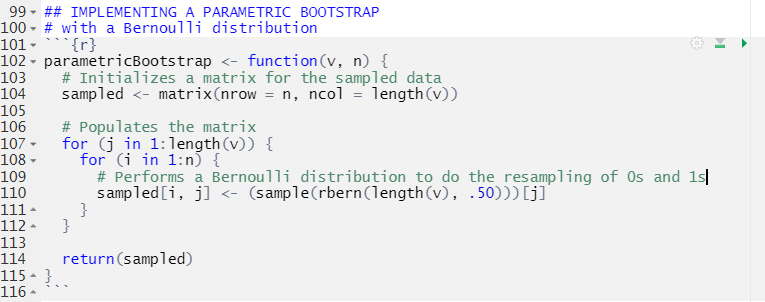
\includegraphics[width=10cm]{ParametricBootstrapCode.png}
\caption{Code to perform a Parametric Resampling on the data given}
\label{fig: Parametric Bootstrap Code}
\end{figure}

\begin{figure}[!hb]
\centering
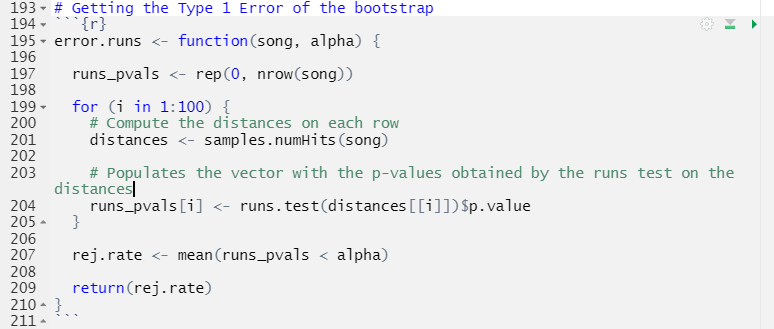
\includegraphics[width=10cm]{Type1ErrCode.png}
\caption{Code to get the Type 1 error of the inputted song}
\label{fig: Type 1 Error Code}
\end{figure}

\begin{figure}
\centering
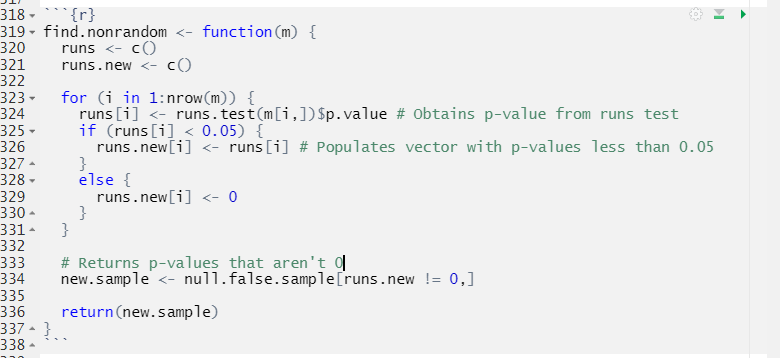
\includegraphics[width=10cm]{FindNonRandomCode.png}
\caption{Code finds the songs that are not random within the matrix}
\label{fig: Find Nonrandom Songs Code}
\end{figure}

\begin{figure}
\centering
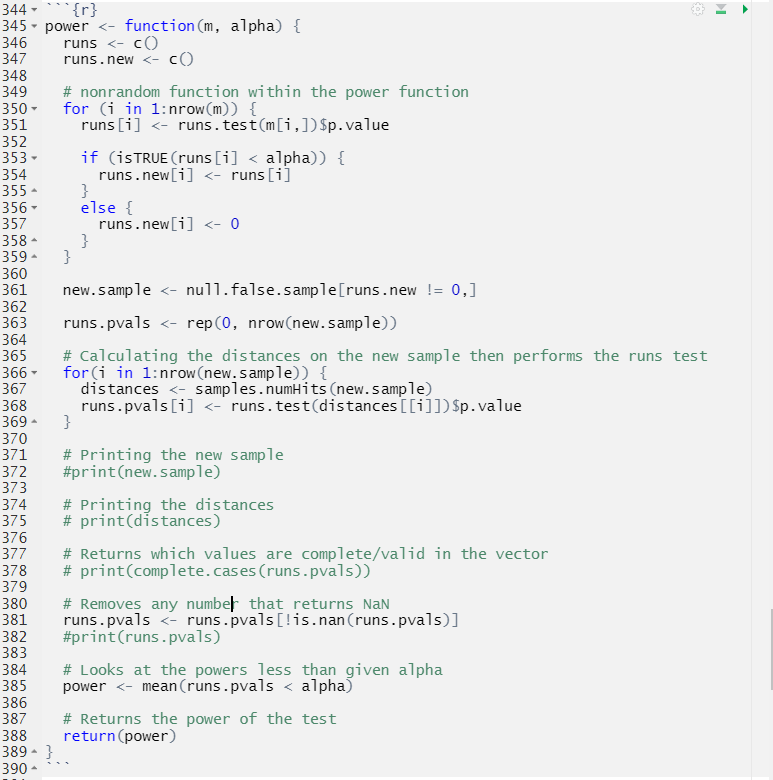
\includegraphics[width=10cm]{PowerCode.png}
\caption{Calculates the power of the test being performed on the song}
\label{fig: Power Code}
\end{figure}


\section{PERSONAL REFLECTIONS}
\subsection{Brianna Cirillo}
\subsection{Samantha Colucci}
\subsection{Shannon Coyle}
From this course, I've definitely gained more knowledge about R Studio and how to perform functions, equations, and other features along with new statistics skills.  In previous courses, I understood the math behind confidence intervals and p-values, but this course truly helped me understand the application and importance of those two components.  It was different learning statistics to apply it to actual data as opposed to just doing the math for homework and tests to get a grade.  When researching, I learned that ideas are not going to work 100\% of the time and that is okay, trial-and-error is an integral part of research that everyone has to go through.  I was also able to learn more from my peers than from the professor because we have a different understanding of topics than a professor does.  I can confidently say that I have a better understanding of statistics after getting explanations from my peers instead of being taught on a whiteboard by someone who has somewhat mastered the topic.  Taking this class has made me more interested in the data science aspect of computer science, whereas, before this course I was on the fence about the crossover between coding and mathematics.  For my future, this course has given me another coding language that I can say that I understand as well as showing me the importance of data and computing.  

I definitely learned a lot about myself by taking this course - both good and bad attributes.  My patience could use some work when it comes to coding, when things would not work the way I wanted to it made me feel like a failure and I would give up.  I did learn that not even the best coders can get these things right the first time.  I also realized that I can work in groups and with whatever I do in my future, I will have to work with others in the technological world.  It was helpful to have Bri and Sam pick me up when I was down and help me understand any of the information that I was struggling to grasp.  They truly helped me with my stress and frustrations, but aside from that, I would take breaks if I found myself getting overly frustrated and remind myself that we were trying to do something that most people will not even attempt in their lifetime.  I was definitely surprised about how I was able to pick up some of the math concepts and then try to figure them out in R.  In the beginning of this class, I was convinced I should not be in it because I felt dumber than everyone else.  After this semester, I've realized that if I should not have been in the class, Dr. B would not have asked me to take it.  I've seen a lot of personal growth this semester, and I am really glad I was able to take this class.  

For the future of this course, I would have mini lessons about the homeworks we did in the beginning of the semester.  I was struggling to fully understand the material and I think having small lessons led by Dr. B would have helped me fully get the topic at hand.  I think the diaries are really important to the course, so I would keep those as well as presenting the homeworks to everyone else in the class.  I think that giving both assignments for the week at the same time would be beneficial if the days between classes aren't that spread out.  One of the hardest parts was finding time to do the second assignment for the week when we only had one full day to complete it.  Other than that, I truly loved this course and I am so glad I was able to take it.  


\end{document}